\section{The big picture}\label{s:lvish-big-picture}

Our library adopts and builds on the basic approach of the @Par@ monad
and the monad-par library~\cite{monad-par}, enabling us to employ our
own notion of lightweight, library-level threads with a custom
scheduler.  It supports the programming model laid out in
Section~\ref{s:quasi-informal} in full, including explicit handler
pools.  It differs from the formalism of Section~\ref{s:quasi-formal}
in following Haskell's by-need evaluation strategy, which also means
that concurrency in the library is \emph{explicitly marked}, either
through uses of a @fork@ function or through asynchronous callbacks,
which run in their own lightweight threads.

\ifdefined\DISSERTATION
\begin{wrapfigure}{l}{1.2in}
\vspace{-2em}
\begin{center}
  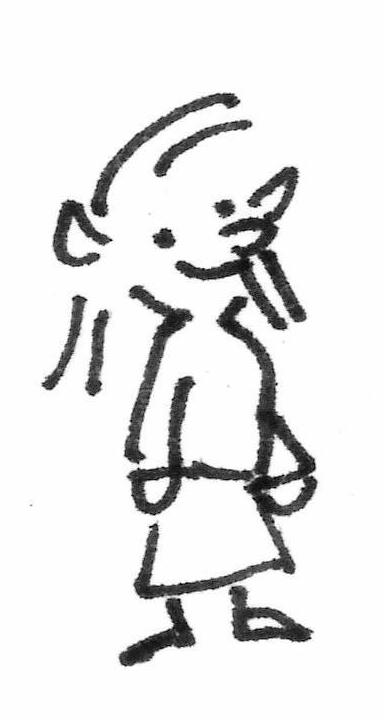
\includegraphics[scale=0.2]{../illustrations/elf}
\end{center}
\vspace{-1.5em}
\end{wrapfigure}
\fi

We envision two parties interacting with the LVish library.  First,
there are \emph{data structure authors}, who use the library directly
to implement a specific monotonic data structure (\eg, a monotonically
growing finite map).  Second, there are \emph{application writers},
who are clients of these data structures.  Only the application
writers receive a \mbox{(quasi-)determinism} guarantee; an author of a
data structure is responsible for ensuring that the states their data
structure can take on correspond to the elements of a lattice, and
that the exposed interface to it corresponds to some use of update
operations, @get@, @freeze@, and event handlers.

The LVish library also includes \emph{lattice-generic} infrastructure:
the @Par@ monad itself, a thread scheduler, support for blocking and
signaling threads, handler pools, and event handlers.  Since this
infrastructure is unsafe---that is, it does not guarantee determinism
or quasi-determinism---only data structure authors should import it,
subsequently exporting a \emph{limited} interface specific to their
data structure.  For finite maps, for instance, this interface might
include key/value insertion, lookup, event handlers and pools, and
freezing---along with higher-level abstractions built on top of these.
Control operators like @fork@ are the only non-data-structure-specific
operations exposed to application writers.

For this approach to scale well with available parallel resources, it
is essential that the data structures themselves support efficient
parallel access; a finite map that was simply protected by a global
lock would force all parallel threads to sequentialize their access.
Thus, we expect data structure authors to draw from the extensive
literature on scalable parallel data structures, employing techniques
like fine-grained locking and lock-free data structures~\cite{art}.
Data structures that fit into the LVish model have a special
advantage: because all updates must commute, it may be possible to
avoid the expensive synchronization which \emph{must} be used for
non-commutative operations~\cite{lawsOfOrder}.  And in any case,
monotonic data structures can be simpler to represent and
implement than general ones.
